\documentclass[10pt]{beamer}
\usetheme{Madrid}
\definecolor{yellow}{RGB}{250, 110, 0}
\setbeamercolor{structure}{fg=yellow}
\setbeamertemplate{footline}[page number]
\setbeamertemplate{caption}[numbered]
\setlength{\parindent}{0.6cm}

\usepackage[utf8]{inputenc}
\usepackage[english]{babel}
\usepackage{amsfonts}
\usepackage{amsmath}
\usepackage{amssymb}
\usepackage{graphicx}
\usepackage{booktabs}
\usepackage{tikz} 
\usepackage{subcaption}
\graphicspath{{Figures/}}

% --- Información de la Portada ---
\title{Large-Signal Analysis of the \textit{CMOS} Differential Pair}
\subtitle{Undergrad \textit{CMOS} Course}
\author{Monja, Ernesto Joaquín}
\institute{Fundación Fulgor}
\date{\today}

\begin{document}

% --- Portada---
\begin{frame}
    \titlepage
    \begin{center}
        \vspace{-0.5cm}
        
\includegraphics[width=6cm]{Fulgor Logo.png}
    \end{center}
\end{frame}


% --- Índice ---
\begin{frame}{Index}
    \tableofcontents
\end{frame}


% --- Introducction:
\section{Initial Thoughts}
\subsection{Why do we need to study Differential Amplifiers?}
\begin{frame}{Why do we need to study Differential Amplifiers?}
    The elegant concept of ''\textit{differential}'' signals and amplifiers was invented in the $1940$’s and first utilized in vacuum-tube circuits. Since then, differential circuits have found increasingly wider usage in microelectronics and serve as a robust, high-performance design paradigm in many of today’s systems. 
    \begin{figure}[H]
        \centering
        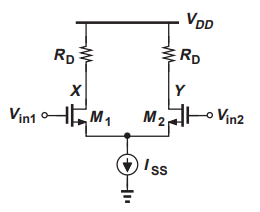
\includegraphics[width=0.27\linewidth]{Figure 1.png}
        \caption{\textit{MOS} Differential Amplifier. \cite{b1}}
        \label{fig:fig_1}
    \end{figure}
    
    In Fig. (\ref{fig:fig_1}), we can see the \textit{MOS} Differential Amplifier that we'll be studying in this presentation.
\end{frame}


\subsection{Introductory Example}
\begin{frame}{Introductory Example}
    We know that \textit{OPAMP's} have $2$ inputs, a point of contrast to the amplifiers studied in previous classes of this course. In order to further understand the need for differential circuits, let us first consider an introductory example.
    
    \begin{block}{Example 1:}
        Let's suppose that a fellow classmate constructs the circuit shown in Fig. \ref{fig:fig_2} to amplify the signal produced by a microphone. Unfortunately, upon applying the result to a speaker, the classmate observes that the amplifier output contains a strong \textit{“humming”} noise, this being a steady low-frequency component. Explain what happens.
    \end{block}
    
    \begin{figure}[H]
        \centering
        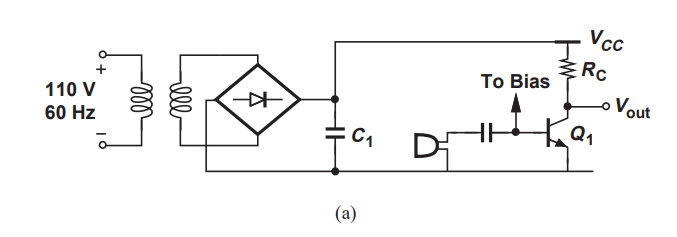
\includegraphics[width=0.6\linewidth]{Figure 2.png}
        \caption{Microphone amplifier designed by a fellow classmate. \cite{b2}}
        \label{fig:fig_2}
    \end{figure}
\end{frame}


\subsection{Understanding the Problem}
\begin{frame}{Introductory Example: Understanding the Problem}
    The current drawn from the rectified output creates a ripple waveform at twice the \textit{AC} line frequency ($50$ or $60 \, [Hz]$) as shown in Fig. (\ref{fig:fig_3}.b)
    \begin{figure}[H]
        \centering
        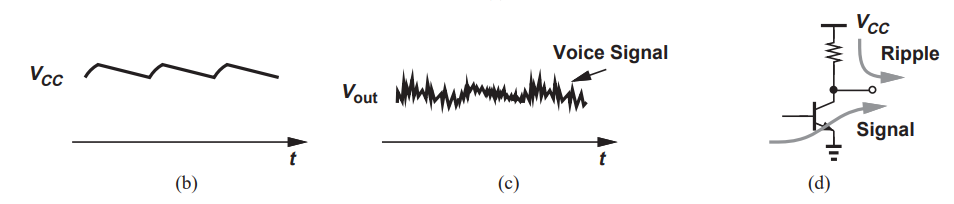
\includegraphics[width=0.7\linewidth]{Figure 3.png}
        \caption{Microphone amplifier designed by a fellow classmate. \cite{b2}}
        \label{fig:fig_3}
    \end{figure}
    
    Examining the output of the common-emitter stage, we can identify two components:
    \begin{itemize}
        \item 1) The amplified version of the microphone signal.
        \item 2) The ripple waveform present on $V_{CC}$.
        \end{itemize}
    
    For the latter, we can write:
    \begin{equation}
        V_{out} = V_{CC} - I_{C} \cdot R_{C}
        \label{eq_1}
    \end{equation}
\end{frame}



\begin{frame}{Introductory Example: Understanding the Problem}
    Noting that $V_{out}$ simply “tracks” $V_{CC}$ in Eq. (\ref{eq_1}) and hence contains the ripple in its entirety. Note also that the “hum” originates from the ripple.
    \begin{figure}[H]
        \centering
        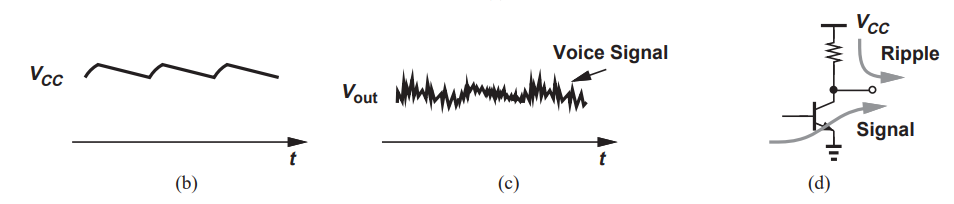
\includegraphics[width=0.8\linewidth]{Figure 3.png}
        \caption{Microphone amplifier designed by a fellow classmate. \cite{b2}}
        \label{fig:fig_4}
    \end{figure}
    
    Fig. (\ref{fig:fig_4}.c) depicts the overall output in the presence of both the signal and the ripple. Illustrated in Fig. (\ref{fig:fig_4}.d), this phenomenon is summarized as the “supply noise goes to the output with a gain of unity.” 
    
    Note that a \textbf{MOS implementation would suffer from the same problem}. Therefore, we wonder: How should we suppress the hum in the above example? 
\end{frame}



\subsection{How to Fix it?}
\begin{frame}{Introductory Example: How to fix it?}
    \begin{block}{Solution 1:}
        We can try increasing $C_{1}$, thus lowering the ripple amplitude, but the required capacitor value may become prohibitively large if many circuits draw current from the rectifier. $\longrightarrow$ \color{red}{NOT} \color{red}{RELIABLE}
    \end{block}

    \vspace{0.1cm}

    \begin{block}{Solution 2:}
        We can modify the amplifier topology such that the output is insensitive to $V_{CC}$.
        \begin{itemize}
            \item Eq. (\ref{eq_1}) implies that a change in $V_{CC}$ directly appears in $V_{out}$, fundamentally because both $V_{out}$ and $V_{CC}$ are measured with respect to ground and differ by a factor of $I_{C}R_{C}$.
            \item But what if $V_{out}$ is not “referenced” to ground? More specifically, what if $V_{out}$ is measured with respect to another point that itself experiences the supply ripple to the same extent? It is thus possible to eliminate the ripple from the “net” output.
        \end{itemize}
        \begin{center}
            \color{green}{COULD WORK!}
        \end{center}
    \end{block}
\end{frame}



\subsection{The Solution}
\begin{frame}{Introductory Example: The Solution}
    While rather abstract, the above conjecture can be readily implemented as shown in Fig. (\ref{fig:fig_5}.a) which illustrates the core concept of the solution to this problem.
    \begin{figure}[H]
        \centering
        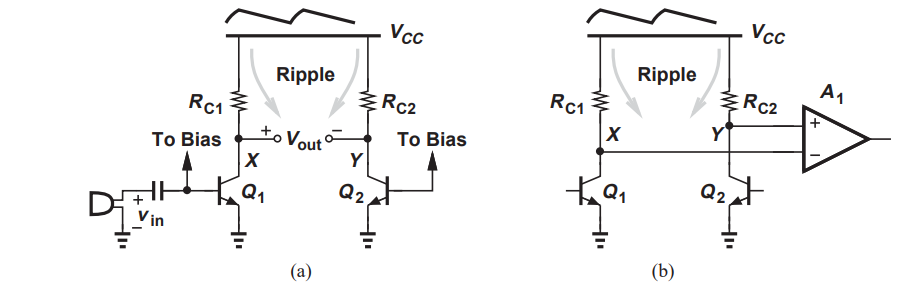
\includegraphics[width=0.9\linewidth]{Figure 5.png}
        \caption{Solution to the \textit{humming} problem. \cite{b3}}
        \label{fig:fig_5}
    \end{figure}
    
    The $CE$ (or $CS$ for MOS amplifiers) stage is duplicated on the right, and the output is now measured between nodes $X$ and $Y$ rather than from $X$ to ground.
\end{frame}



\begin{frame}{Introductory Example: The Solution}
    One may wonder then: \textit{what happens if} $V_{CC}$ \textit{contains ripple?} Well, note that both $V_{X}$ and $V_{Y}$ rise and fall by the same amount and hence the difference between $V_{X}$ and $V_{Y}$ remains free from the ripple.
    
    In fact, denoting the ripple by $v_{r}$, we express the small-signal voltages at these
    nodes as:
    \begin{equation}
        \begin{cases}
            v_{X} = A_{v} \cdot v_{in} + v_{r} \\
            v_{Y} = v_{r}
        \end{cases}
        \label{eq_2}
    \end{equation}
    
    That is:
    \begin{equation}
        v_{X} - v_{Y} = A_{v} \cdot v_{in}
        \label{eq_3}
    \end{equation}
    
    Note that $Q_2$ carries no signal, simply serving as a constant current source. The above development serves as the foundation for \textbf{differential amplifiers}: the symmetric CE stages provide two output nodes whose voltage difference remains free from the supply ripple.
\end{frame}



\section{Differential Amplifier}
\subsection{Analysis of the Solution}
\begin{frame}{Differential Signals: Analysis of the Solution}
    Let us return to the circuit of Fig. (\ref{fig:fig_5}.a) and recall that the duplicate stage consisting of $Q_{2}$ and $R_{C2}$ remains “idle”, thereby “wasting” current. 
    
    We may therefore wonder if this stage can provide signal amplification in addition to establishing a reference point for $V_{out}$.  In our first attempt, we directly apply the input signal to the base of $Q_{2}$ as shown in Fig. (\ref{fig:fig_6}.a).
    \begin{figure}[H]
        \centering
        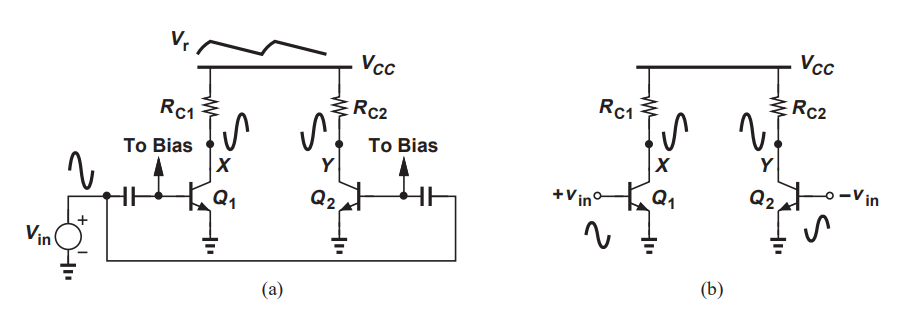
\includegraphics[width=0.8\linewidth]{Figure 6.png}
        \caption{(a) Application of one input signal to two CE stages, (b) use of differential input signals. \cite{b4}}
        \label{fig:fig_6}
    \end{figure}
\end{frame}


\subsection{An improvement of the solution}
\begin{frame}{Differential Signals: An improvement of the solution}
    Unfortunately, the signal components at X and Y are in phase, canceling each other as
    they appear in $v_{X} - v_{Y}$:
    \begin{equation}
        \begin{cases}
            v_{X} = A_{v} \cdot v_{in} + v_{r} \\
            v_{Y} = A_{v} \cdot v_{in} + v_{r}
        \end{cases}
        \label{eq_4}
    \end{equation}
    
    For the signal components to enhance each other at the output, we can invert one of
    the input phases as shown in Fig. (\ref{fig:fig_6}.b), obtaining:
    \begin{equation}
        \begin{cases}
            v_{X} = A_{v} \cdot v_{in} + v_{r} \\
            v_{Y} = - A_{v} \cdot v_{in} + v_{r}
        \end{cases}
        \label{eq_5}
    \end{equation}
    
    and hence
    \begin{equation}
        v_{X} - v_{Y} = 2 \cdot A_{v} v_{in}
        \label{eq_6}
    \end{equation}
    
    Compared to the circuit of Fig. (\ref{fig:fig_5}.a), this topology provides twice the output swing by exploiting the amplification capability of the duplicate stage.
\end{frame}


\subsection{Waveform Analysis}
\begin{frame}{Differential Signals: Waveform Analysis}
    Our thought process has led us to the specific waveforms in Fig. (\ref{fig:fig_6}.b): the circuit senses $2$ inputs that vary by equal and opposite amounts and generates $2$ outputs that behave in a similar fashion. 
    
    These waveforms are examples of \textbf{“differential”} signals and stand in contrast to \textbf{“single-ended”} signals —the type to which we are accustomed from basic circuits and previous classes of this course.
    
    More specifically, a single-ended signal is one measured with respect to the common ground (Fig. (\ref{fig:fig_7}.a)) and “carried by one line”, whereas a differential signal is measured between two nodes that have equal and opposite swings (Fig. (\ref{fig:fig_7}.b)) and is thus “carried by two lines”.
    \begin{figure}[H]
        \centering
        \begin{subfigure}[b]{0.35\linewidth}
            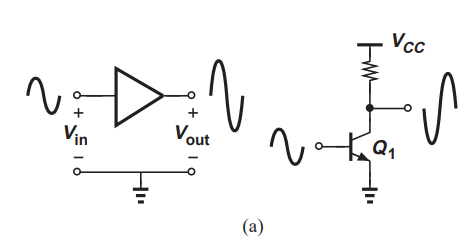
\includegraphics[width=\linewidth]{Figure 7.1.png}
        \end{subfigure}
        \begin{subfigure}[b]{0.45\linewidth}
            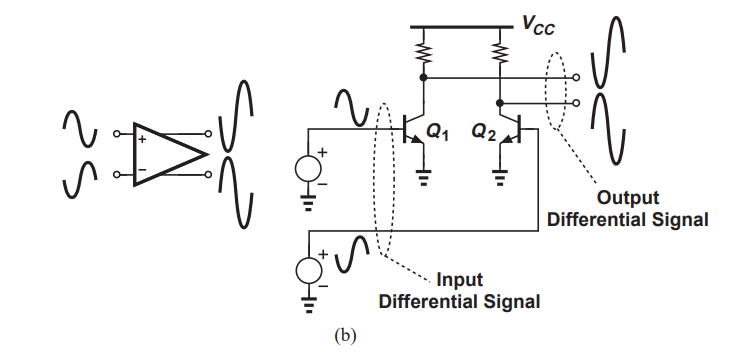
\includegraphics[width=\linewidth]{Figure 7.2.png}
        \end{subfigure}
        \caption{a) Single-ended signals, b) Differential signals. \cite{b5}}
        \label{fig:fig_7}
    \end{figure}
\end{frame}



\begin{frame}{Differential Signals: Waveform Analysis}
    Here, $V_{1}$ and $V_{2}$ vary by equal and opposite amounts and have the same average (\textit{DC}) level, $V_{CM}$, with respect to ground:
    \begin{equation}
        \begin{cases}
            V_{1} = V_{0} \cdot \sin(\omega t) + V_{CM} \\
            V_{2} = -V_{0} \cdot \sin(\omega t) + V_{CM}
        \end{cases}
    \end{equation}
    
    The \textit{DC} voltage that is common to both $V_{1}$ and $V_{2}$ is called the \textbf{“common-} \textbf{mode (CM) level”}. That is, in the absence of differential signals, the $2$ nodes remain at a potential equal to $V_{CM}$ with respect to the global ground (see Fig. (\ref{fig:fig_8})).
    \begin{figure}[H]
        \centering
        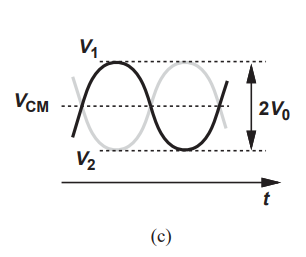
\includegraphics[width=0.25\linewidth]{Figure 8.png}
        \caption{Illustration of common-mode level. \cite{b5}}
        \label{fig:fig_8}
    \end{figure}
\end{frame}



\section{CMOS Differential Pair}
\subsection{Tail current source.}
\begin{frame}{CMOS Differential Pair: Tail current source}
    Before formally introducing the differential pair, we must recognize that the circuit of
    Fig. (\ref{fig:fig_7}.b) senses $2$ inputs and can therefore serve as $A_{1}$ in Fig. (\ref{fig:fig_5}.b). This observation leads to the differential pair.
    
    While sensing and producing differential signals, the circuit of Fig. (\ref{fig:fig_7}.b) suffers from some drawbacks. Fortunately, a simple modification yields an elegant, versatile topology: the sources of $M_{1}$ and $M_{2}$ are tied to a constant current source rather than to ground that we call $I_{SS}$ - the “tail current source” as shown in Fig. (\ref{fig:fig_9}).
    \begin{figure}[H]
        \centering
        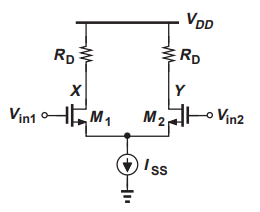
\includegraphics[width=0.27\linewidth]{Figure 1.png}
        \caption{\textit{MOS} Differential Amplifier. \cite{b1}}
        \label{fig:fig_9}
    \end{figure}
\end{frame}



\subsection{Qualitative Analysis}
\begin{frame}{CMOS Differential Pair: Qualitative Analysis}
    \begin{figure}[H]
        \centering
        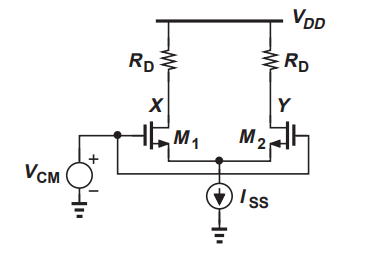
\includegraphics[width=0.3\linewidth]{Figure 10.png}
        \caption{Response of MOS differential pair to input CM variation. \cite{b6}}
        \label{fig:fig_10}
    \end{figure}
    
    Fig. (\ref{fig:fig_10}) depicts the \textit{MOS} pair with the two inputs tied to $V_{CM}$, where if we assume perfect symmetry, we have:
    \begin{equation}
        I_{D1} = I_{D2} = \frac{I_{SS}}{2}
        \label{eq_8}
    \end{equation}
    
    and:
    \begin{equation}
        V_{X} = V_{Y} = V_{DD} - \frac{I_{SS}}{2} \cdot R_{D}
        \label{eq_9}
    \end{equation}
\end{frame}



\begin{frame}{CMOS Differential Pair: Qualitative Analysis}
    Eq. (\ref{eq_9}) shows that a zero differential input gives a zero differential output. Note that the output common mode level is equal to: $V_{DD} - R_{D} \cdot I_{SS}/2 $.
    
    For our subsequent derivations, it is useful to compute the \textit{“equilibrium overdrive voltage”} of $M_{1}$ and $M_{2}$, $(V_{GS} - V_{Th})_{equil}$. We assume $\lambda = 0$ and hence:
    \begin{equation}
        I_{D} = \frac{1}{2} \mu_{n} C_{ox} \left(\frac{W}{L}\right) (V_{GS} - V_{Th})^{2}
        \label{eq_10}
    \end{equation}
    
    Carrying a current of $I_{SS}/2$, each device exhibits an overdrive of:
    \begin{equation}
        (V_{GS} - V_{Th})_{equil} = \sqrt{\frac{I_{SS}}{\mu_{n} C_{ox} \left(\frac{W}{L}\right)}} 
        \label{eq_11}
    \end{equation}
    
    As expected, a greater tail current or a smaller $W/L$ translates to a larger equilibrium
    overdrive.
\end{frame}



\begin{frame}{CMOS Differential Pair: Qualitative Analysis}
    To guarantee that $M_{1}$ and $M_{2}$ operate in saturation, we require that their drain voltages
    not fall below: $V_{CM} - V_{Th}$:
    \begin{equation}
        V_{DS} = V_{DD} - R_{D} \cdot \frac{I_{SS}}{2} > V_{CM} - V_{Th}
        \label{eq_12}
    \end{equation}
    
    It can also be observed that a change in $V_{CM}$ cannot alter $I_{D1} = I_{D2} = I_{SS}/2$, leaving $V_{X}$ and $V_{Y}$ undisturbed. The circuit thus rejects input CM variations.
    
    \vspace{1cm}
    \begin{center}
        \textbf{and what about the Differential Mode?}
    \end{center}
\end{frame}



\begin{frame}{CMOS Differential Pair: Qualitative Analysis}
    \begin{figure}[H]
        \centering
        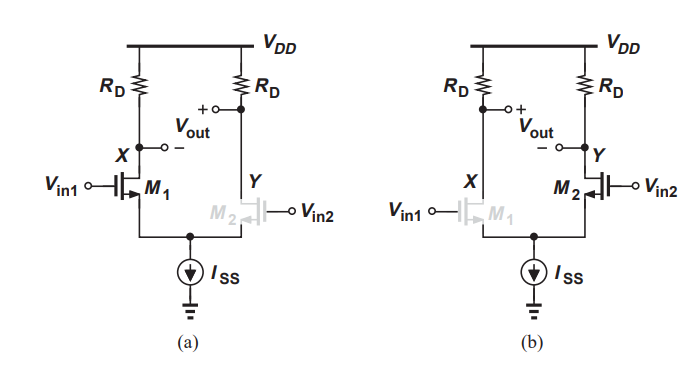
\includegraphics[width=0.55\linewidth]{Figure 11.png}
        \caption{(a) Response of \textit{MOS} differential pair to very positive input, (b) response of \textit{MOS} differential pair to very negative input. \cite{b7}}
        \label{fig:fig_11}
    \end{figure}
    
    Fig. (\ref{fig:fig_11}) illustrates the response of the \textit{MOS} pair to large differential inputs. If $V_{in1}$ is well above $V_{in2}$ [Fig. (\ref{fig:fig_11}.a)], then $M_{1}$ carries the entire tail current, generating:
    \begin{equation}
        \begin{cases}
            V_{X} = V_{DD} - I_{SS} \cdot R_{D} \\
            V_{Y} = V_{DD}
        \end{cases}
        \label{eq_13}
    \end{equation}
\end{frame}



\begin{frame}{CMOS Differential Pair: Qualitative Analysis}
    Similarly, if $V_{in2}$ is well above $V_{in1}$ [Fig. (\ref{fig:fig_11}.b)], then
    \begin{equation}
        \begin{cases}
            V_{X} = V_{DD} \\
            V_{Y} = V_{DD} - I_{SS} \cdot R_{D}
        \end{cases}
        \label{eq_14}
    \end{equation}
    
    The circuit therefore steers the tail current from one side to the other, producing a differential output in response to a differential input. Figure (\ref{fig:fig_12}.c) sketches the characteristics of the circuit.
    \begin{figure}[H]
        \centering
        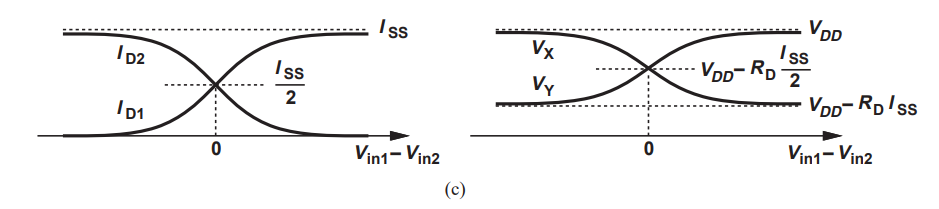
\includegraphics[width=0.8\linewidth]{Figure 12.png}
        \caption{Qualitative plots of currents and voltages. \cite{b7}}
        \label{fig:fig_12}
    \end{figure}
\end{frame}



\begin{frame}{CMOS Differential Pair: Qualitative Analysis}
    Let us now examine the circuit’s behavior for a small input difference depicted in
    Fig. (\ref{fig:fig_13}). 
    \begin{figure}[H]
        \centering
        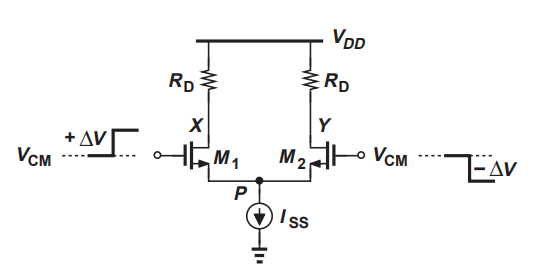
\includegraphics[width=0.4\linewidth]{Figure 13.png}
        \caption{Qualitative plots of currents and voltages. \cite{b8}}
        \label{fig:fig_13}
    \end{figure}
    
    In such scenario, the gate voltage of $M_{1}$ is raised from $V_{CM}$ by $\Delta V$ while that of
    $M_{2}$ is lowered from $V_{CM}$ by the same amount. We surmise that $I_{D1}$ increases slightly and, since: $I_{D1} + I_{D2} = I_{SS}$, $I_{D2}$ decreases by the same amount:
    \begin{equation}
        \begin{cases}
            I_{D1} = \frac{I_{SS}}{2} + \Delta I \\
            I_{D2} = \frac{I_{SS}}{2} - \Delta I
        \end{cases}
        \label{eq_15}
    \end{equation}
\end{frame}



\begin{frame}{CMOS Differential Pair: Qualitative Analysis}
    Now one may wonder how is $\Delta I$ related to $\Delta V$? If the sources of $M_{1}$ and $M_{2}$ were directly tied to ground, then $\Delta I$ would simply be equal to: $g_m \Delta V$. In the differential pair, however, node P is free to rise or fall. We must therefore compute the change in $V_{P}$.
    
    Suppose $V_{P}$ rises by $\Delta V_{P}$. As a result, the net increase in $V_{GS1}$ is equal to $\Delta V - \Delta V_{P}$ and hence:
    \begin{equation}
        \Delta I_{D1} = g_{m}(\Delta V - \Delta V_{P})
        \label{eq_16}
    \end{equation}
    
    Similarly, the net decrease in $V_{GS2}$ is equal to $\Delta V + \Delta V_{P}$, yielding:
    \begin{equation}
        \Delta I_{D2} = -g_{m}(\Delta V + \Delta V_{P})
        \label{eq_17}
    \end{equation}
    
    But recall from Eq. (\ref{eq_15}) that $\Delta I_{D1}$ must be equal to $-\Delta I_{D2}$, dictating that:
    \begin{equation}
        g_{m}(\Delta V - \Delta V_{P}) = -g_{m}(\Delta V + \Delta V_{P}) \xrightarrow{} \Delta V_{P} = 0
        \label{eq_18}
    \end{equation}
\end{frame}



\begin{frame}{CMOS Differential Pair: Qualitative Analysis}
    Therefore, it follows that:
    \begin{equation}
        \begin{cases}
            \Delta I_{D1} =   g_{m} \Delta V \\
            \Delta I_{D2} = - g_{m} \Delta V
        \end{cases}
        \label{eq_19}
    \end{equation}
    
    and:
    \begin{equation}
        \begin{cases}
            \Delta V_{X} =   g_{m} \Delta V R_{D}\\
            \Delta V_{Y} = - g_{m} \Delta V R_{D}
        \end{cases}
        \label{eq_20}
    \end{equation}

    The differential output therefore goes from $0$ to:
    \begin{equation}
        \Delta V_{X} - \Delta V_{Y} = -2 g_{m} R_{D} \Delta V
        \label{eq_21}
    \end{equation}
    
    We define the small-signal differential gain of the circuit as:
    \begin{equation}
        A_{v} = \frac{\text{Change in Differential Output}}{\text{Change in Differential Input}} = \frac{-2 g_{m} R_{D} \Delta V}{2 \Delta V} = -g_{m} R_{D}
        \label{eq_22}
    \end{equation}
    
    This expression is similar to that of the \textit{common-source stage}.
    % (Note that the change in the differential input is equal to $2 \Delta V$.) 
\end{frame}


\subsection{Large-Signal Analysis}
\begin{frame}{CMOS Differential Pair: Large-Signal Analysis}
    Our objective here is to derive the input/output characteristics of the \textit{MOS} pair as the differential input varies from very negative to very positive values. From Fig. (\ref{fig:fig_14}),
    we have:
    \begin{equation}
        V_{out} = V_{out1} - V_{out2} = -R_{D}(I_{D1} - I_{D2})
        \label{eq_23}
    \end{equation}
    
    \begin{figure}[H]
        \centering
        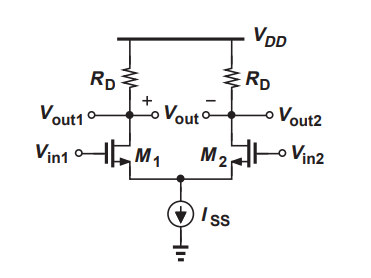
\includegraphics[width=0.35\linewidth]{Figure 14.png}
        \caption{MOS differential pair for large-signal analysis. \cite{b9}}
        \label{fig:fig_14}
    \end{figure}
\end{frame}



\begin{frame}{CMOS Differential Pair: Large-Signal Analysis}
    To obtain $I_{D1} - I_{D2}$, we neglect channel-length modulation and write a \textit{KVL} around the input network and a \textit{KCL} at the tail node:
    \begin{equation}
        V_{in1} - V_{GS1} = V_{in2} - V_{GS2}
        \label{eq_24}
    \end{equation}
    \begin{equation}
        I_{D1} + I_{D2} = I_{SS}
        \label{eq_25}
    \end{equation}
    
    Since $I_{D} = (1/2) \mu_{n} C_{ox} (W/L) (V_{GS} - V_{Th})^{2}$, we have:
    \begin{equation}
        V_{GS} = V_{Th} + \sqrt{\frac{2 I_{D}}{\mu_{n} C_{ox} \frac{W}{L}}}
        \label{eq_26}
    \end{equation}
    
    Substituting for $V_{GS1}$ and $V_{GS2}$ in Eq. (\ref{eq_24}), we have:
    \begin{equation}
        V_{in1} - V_{in2} = V_{GS1} - V_{GS2}
        \label{eq_27}
    \end{equation}
    \begin{equation}
        V_{in1} - V_{in2} = \sqrt{\frac{2}{\mu_{n} C_{ox} \frac{W}{L}}} (\sqrt{I_{D1}} - \sqrt{I_{D2}})
        \label{eq_28}
    \end{equation}
\end{frame}



\begin{frame}{CMOS Differential Pair: Large-Signal Analysis}
    Squaring both sides yields:
    \begin{equation}
        (V_{in1} - V_{in2})^{2} = \frac{2}{\mu_{n} C_{ox} \frac{W}{L}} (I_{D1} + I_{D2} - 2\sqrt{I_{D1}I_{D2}})
        \label{eq_29}
    \end{equation}

    Recognizing that $I_{D1} + I_{D2} = I_{SS}$, we obtain:
    \begin{equation}
        (V_{in1} - V_{in2})^{2} = \frac{2}{\mu_{n} C_{ox} \frac{W}{L}} (I_{SS} - 2\sqrt{I_{D1}I_{D2}})
        \label{eq_30}
    \end{equation}
    
    We now find $\sqrt{I_{D1}I_{D2}}$,
    \begin{equation}
        4\sqrt{I_{D1}I_{D2}} = 2I_{SS} - \mu_{n} C_{ox} \frac{W}{L} (V_{in1} - V_{in2})^{2}
        \label{eq_31}
    \end{equation}
    
    square the result again,
    \begin{equation}
        16I_{D1}I_{D2} = \left[ 2I_{SS} - \mu_{n} C_{ox} \frac{W}{L} (V_{in1} - V_{in2})^{2} \right]^{2}
        \label{eq_32}
    \end{equation}
\end{frame}



\begin{frame}{CMOS Differential Pair: Large-Signal Analysis}
    and substitute $I_{SS} - I_{D1}$ for $I_{D2}$,
    \begin{equation}
        16I_{D1}(I_{SS} - I_{D1}) = \left[ 2I_{SS} - \mu_{n} C_{ox} \frac{W}{L} (V_{in1} - V_{in2})^{2} \right]^{2}
        \label{eq_33}
    \end{equation}
    
    It follows that:
    \begin{equation}
        16I_{D1}^{2} - 16I_{SS}I_{D1} + \left[ 2I_{SS} - \mu_{n} C_{ox} \frac{W}{L} (V_{in1} - V_{in2})^{2} \right]^{2} = 0
        \label{eq_34}
    \end{equation}
    
    and solving the quadratic expression, we have:
    \begin{equation}
        I_{D1} = \frac{I_{SS}}{2} \pm \frac{1}{4} \sqrt{4I_{SS}^{2} - \left[\mu_{n} C_{ox} \frac{W}{L}(V_{in1} - V_{in2})^{2} -2I_{SS}\right]^2}
        \label{eq_35}
    \end{equation}
    
    Note that the only solution that is valid, is the one with the sum of the two terms:
    \begin{equation}
        I_{D1} = \frac{I_{SS}}{2} + \frac{V_{in1} - V_{in2}}{4} \sqrt{\mu_{n} C_{ox} \frac{W}{L} \left[4I_{SS} - \mu_{n} C_{ox} \frac{W}{L} (V_{in1} - V_{in2})^{2}\right]}
        \label{eq_36}
    \end{equation}
\end{frame}



\begin{frame}{CMOS Differential Pair: Large-Signal Analysis}
    The symmetry of the circuit also implies that:
    \begin{equation}
        I_{D2} = \frac{I_{SS}}{2} + \frac{V_{in2} - V_{in1}}{4} \sqrt{\mu_{n} C_{ox} \frac{W}{L} \left[4I_{SS} - \mu_{n} C_{ox} \frac{W}{L} (V_{in2} - V_{in1})^{2}\right]}
        \label{eq_37}
    \end{equation}
    
    That is,
    \begin{equation}
        I_{D1} - I_{D2} = \frac{1}{2} \mu_{n} C_{ox} \frac{W}{L} (V_{in1} - V_{in2}) \sqrt{\frac{4I_{SS}}{\mu_{n} C_{ox} \frac{W}{L}} - (V_{in1} - V_{in2})^2}
        \label{eq_38}
    \end{equation}
    
    Where Eqs. (\ref{eq_36}) - (\ref{eq_38}) form the foundation of our understanding of the \textit{MOS} differential pair
\end{frame}



\begin{frame}{CMOS Differential Pair: Large-Signal Analysis}
    Let us now examine Eq. (\ref{eq_38}) closely.
    \begin{itemize}
        \item As expected from the characteristics in Fig. (\ref{fig:fig_15}.c), the right-hand side is an odd (symmetric) function of $V_{in1} - V_{in2}$, dropping to zero for a zero input difference.
        \begin{figure}[H]
            \centering
            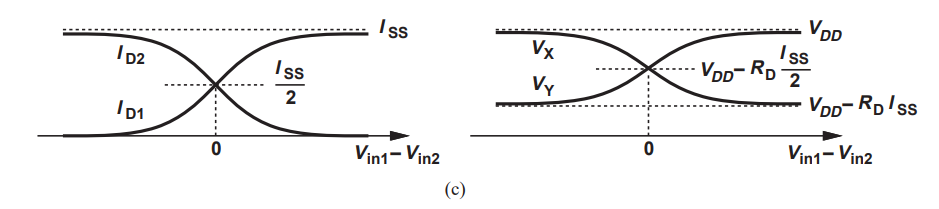
\includegraphics[width=0.7\linewidth]{Figure 12.png}
            \caption{Qualitative plots of currents and voltages. \cite{b7}}
            \label{fig:fig_15}
        \end{figure}
        
        \item But, \textit{can the difference under the square root vanish, too?} That would suggest that: $I_{D1} - I_{D2}$ falls to zero as $(V_{in1} - V_{in2})^{2}$ reaches $4I_{SS}/(\mu_{n} C_{ox} W/L)$, an effect not predicted by our qualitative sketches in  Fig. (\ref{fig:fig_15}.c). Furthermore, it appears that the argument of the square root becomes negative as $(V_{in1} - V_{in2})^{2}$  exceeds this value! $\xrightarrow{}$ \textbf{How should these results be interpreted?}
    \end{itemize}
\end{frame}



\begin{frame}{CMOS Differential Pair: Large-Signal Analysis}
    \begin{itemize}
        \item Implicit in our foregoing derivations is the assumption both transistors are on. However, as $|V_{in1} - V_{in2}|$ rises, at some point $M_{1}$ or $M_{2}$ turns off, violating the above equations.

        \item We must therefore determine the input difference that places one of the transistors at the edge of conduction.
        \begin{itemize}
            \item This can be accomplished by equating Eqs. (\ref{eq_36}) and (\ref{eq_37}), or (\ref{eq_38}) to $I_{SS}$, but this leads to lengthy algebra...
            
            \item Instead, we recognize from Fig. (\ref{fig:fig_16}) that if, for example, $M_{1}$ approaches the edge of conduction, then its gate-source voltage falls to a value equal to $V_{Th}$.
        \end{itemize}
    \end{itemize}
    \begin{figure}[H]
        \centering
        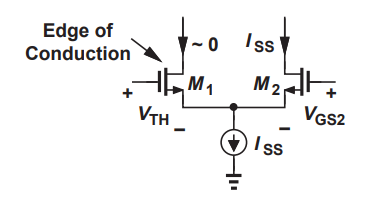
\includegraphics[width=0.5\linewidth]{Figure 16.png}
        \caption{MOS differential pair with one device off. \cite{b10}}
        \label{fig:fig_16}
    \end{figure}
\end{frame}



\begin{frame}{CMOS Differential Pair: Large-Signal Analysis}
     Also, the gate-source voltage of $M_{2}$ must be sufficiently large to accommodate a drain current of $I_{SS}$:
     \begin{equation}
         \begin{cases}
             V_{GS1} = V_{Th} \\
             V_{GS2} = V_{Th} + \sqrt{\frac{2 I_{SS}}{\mu_{n} C_{ox} \frac{W}{L}}}
         \end{cases}
         \label{eq_39}
     \end{equation}

     It follows from Eq. (\ref{eq_24}) that:
     \begin{equation}
         |V_{in1} - V_{in2}|_{max} = \sqrt{\frac{2 I_{SS}}{\mu_{n} C_{ox} \frac{W}{L}}}
         \label{eq_40}
     \end{equation}
     
     \begin{itemize}
         \item where $|V_{in1} - V_{in2}|_{max}$ denotes the input difference that places one transistor at the edge of conduction.
         \item Eq. (\ref{eq_40}) is invalid for input differences greater than this value.
         \item Indeed, substituting from Eq. (\ref{eq_40}) in (\ref{eq_38}) also yields $|I_{D1} - I_{D2}| = I_{SS}$. We also note that $|V_{in1} - V_{in2}|_{max}$ can be related to the equilibrium overdrive [Eq. (\ref{eq_11})] as follows:
         \begin{equation}
             |V_{in1} - V_{in2}|_{max} = \sqrt{2} (V_{GS} - V_{Th})_{equil.}
             \label{eq_41}
         \end{equation}
     \end{itemize}
\end{frame}



\begin{frame}{CMOS Differential Pair: Large-Signal Analysis}
    The above findings are very important and stand in contrast to the behavior of the bipolar differential pair: 
    \begin{itemize}
        \item The \textit{MOS} pair steers all of the tail current for $|V_{in1} - V_{in2}|_{max}$ whereas the bipolar counterpart only approaches this condition for a finite input difference.
        
        \begin{equation}
             |V_{in1} - V_{in2}|_{max} = \sqrt{2} (V_{GS} - V_{Th})_{equil.}
             \label{eq_42}
         \end{equation}
        
        \item Equation (\ref{eq_42}) provides a great deal of intuition into the operation of the \textit{MOS} pair: Specifically, we plot $I_{D1}$ and $I_{D2}$ as in Fig. (\ref{fig:fig_17}.a), where $\Delta V_{in} = V_{in1} - V_{in2}$, arriving at the differential characteristics in Figs. (\ref{fig:fig_17}.b) and (\ref{fig:fig_17}.c). The circuit thus behaves linearly for small values of $\Delta V_{in}$ and becomes completely nonlinear for $\Delta V_{in} > \Delta V_{in,max}$. In other words, $\Delta V_{in,max}$ serves as an absolute bound on the input signal levels that have any effect on the output.
    \end{itemize}
\end{frame}



\begin{frame}{CMOS Differential Pair: Large-Signal Analysis}
    \begin{figure}[H]
        \centering
        \includegraphics[width=0.6\linewidth]{Figuras/Figure 17.png}
        \caption{Variation of (a) drain currents, (b) the difference between drain currents, and (c) differential output voltage as a function of input. \cite{b11}}
        \label{fig:fig_17}
    \end{figure}
\end{frame}



\section{Conclusion}
\begin{frame}{Conclusion}
    \begin{itemize}
        \item Thank you for listening! If you have any questions about the topics in this presentation, feel free to ask and we can discuss them anytime.
    \end{itemize}

    \vspace{0.2cm}
    
    \begin{figure}[H]
        \centering
        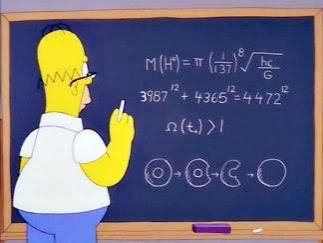
\includegraphics[width=0.5\linewidth]{Thanks.png}
        \caption{Me explaining \textit{MOS} Differential Pairs.}
        \label{fig:fig_18}
    \end{figure}
\end{frame}



\section{Bibliography}
\begin{frame}[allowframebreaks]{Bibliography}
    \begin{thebibliography}{9}
        \bibitem{b1} Behzad Razavi \textit{Fundamentals of Microelectronics}
        \\ {\scriptsize Chapter 10, Figure 10.6 (b) (2026).}

        \vspace{0.1 cm}

        \bibitem{b2} Behzad Razavi \textit{Fundamentals of Microelectronics}
        \\ {\scriptsize Chapter 10, Figure 10.1 (a) (2026).}

        \vspace{0.1 cm}

        \bibitem{b3} Behzad Razavi \textit{Fundamentals of Microelectronics}
        \\ {\scriptsize Chapter 10, Figure 10.2 (2026).}

        \vspace{0.1 cm}

        \bibitem{b4} Behzad Razavi \textit{Fundamentals of Microelectronics}
        \\ {\scriptsize Chapter 10, Figure 10.3 (2026).}

        \vspace{0.1 cm}

        \bibitem{b5} Behzad Razavi \textit{Fundamentals of Microelectronics}
        \\ {\scriptsize Chapter 10, Figure 10.4 (2026).}

        \vspace{0.1 cm}

        \bibitem{b6} Behzad Razavi \textit{Fundamentals of Microelectronics}
        \\ {\scriptsize Chapter 10, Figure 10.24 (2026).}

        \vspace{0.1 cm}

        \bibitem{b7} Behzad Razavi \textit{Fundamentals of Microelectronics}
        \\ {\scriptsize Chapter 10, Figure 10.25 (2026).}

        \vspace{0.1 cm}

        \bibitem{b8} Behzad Razavi \textit{Fundamentals of Microelectronics}
        \\ {\scriptsize Chapter 10, Figure 10.26 (2026).}

        \vspace{0.1 cm}

        \bibitem{b9} Behzad Razavi \textit{Fundamentals of Microelectronics}
        \\ {\scriptsize Chapter 10, Figure 10.29 (2026).}

        \vspace{0.1 cm}

        \bibitem{b10} Behzad Razavi \textit{Fundamentals of Microelectronics}
        \\ {\scriptsize Chapter 10, Figure 10.30 (2026).}

        \vspace{0.1 cm}

        \bibitem{b11} Behzad Razavi \textit{Fundamentals of Microelectronics}
        \\ {\scriptsize Chapter 10, Figure 10.31 (2026).}
    \end{thebibliography}
\end{frame}

\end{document}